\section{Work plan}
We held many meetings throughout the term on the subject of planning and task division. On average, we would meet once every week or two to modify design decisions and evolve the architecture. Whiteboarding of the design and architecture was documented partially through github and partially through the teams slack channel.

\subsection{Timeline}
Cumulatively, we logged 467 hours of work on this prototype. Figure~\ref{fig:work-per-week} shows the week-by-week breakdown. On average, we spent 38.125 hours building the prototype. 

\begin{figure}[tbph]
  \centering
  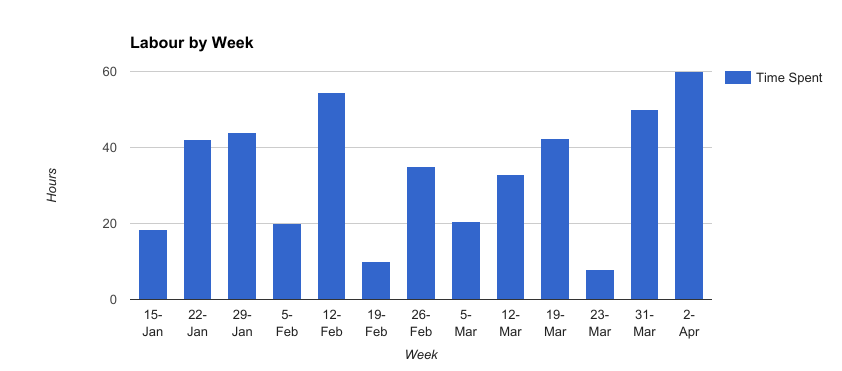
\includegraphics[width=0.85\linewidth]{graphics/work-per-week}
  \caption{Work per week on prototype, all tasks}
  \label{fig:work-per-week}
\end{figure}

It can be clearly seen that work was performed in bursts corresponding to our sprints.  Weeks with many midterms in mid February and March are also notable for their minimal work, this is due to the midterms and other course responsibilities that occurred during these times.

Every week we would meet to keep track of how everyone was doing on their assigned tasks. We kept track of assigned tasks through github issues. This allowed us to view a commit-by-commit snapshot of how the tasks were moving forward, and keep on track to finish within the provided deadline.  Overall while there were some hiccups and time crunches, we were ultimately able to meet all deadlines.

Figure~\ref{fig:work-pie} shows that over half of the work time was spent on implementation. Design sessions took the form of collaborative whiteboarding and brainstorming activities with the group as a whole. 

\begin{figure}[tbph]
  \centering
  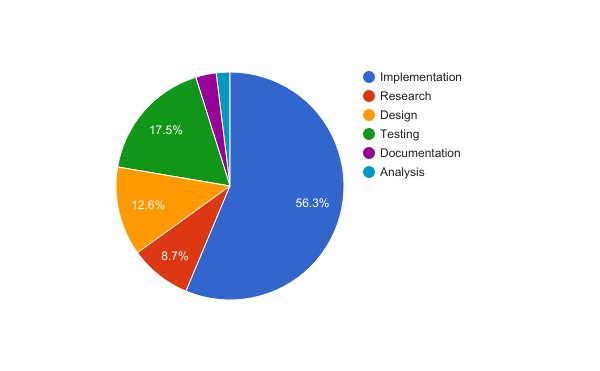
\includegraphics[width=0.8\linewidth]{graphics/work-pie}
  \caption{Areas of work}
  \label{fig:work-pie}
\end{figure}

The categories are defined as:

\begin{itemize}
  \item \textit{Analysis}: The profiling and measurement of code and project performance
  \item \textit{Design}: Architecture discussions and whiteboarding
  \item \textit{Documentation}: The recording of work and design
  \item \textit{Implementation}: The writing of code, building of custom tools, setup of environments and off the shelf components
  \item \textit{Research}: The learning of tools, technologies, as well as background research into domains and tools
  \item \textit{Testing}: Ensuring the code works correctly and to spec.
\end{itemize}

Of the total time spent creating the day trading systems, slightly more than three quarters of the time was spent on actual implementation, with the next largest category being testing.  Our group's total development time was much higher than that of either group one or two, and while we achieved the highest performance we believe that our total implementation time was disproportionately large compared to what it could have been.  Development time could have been minimized had the implementation of specific features been planned more thoroughly.  Had more time been dedicated to team meetings, discussion, and architecture planning it is highly likely that we could have achieved a 2:1 ROI on our time investment by drastically reducing rewrites.  Additionally an additional investment into documentation would likely have also reduced the amount of time spent on knowledge transfer and reverse engineering other team mates work.  It is our team’s recommendation that future groups invest dedicated time to design and documentation as opposed to treating them as secondary requirements to building.



